%!TEX root = ../paper.tex
\section{Einleitung}

Mixed Reality (MR) Techniken finden sich neben dem Einsatz in der Spiele-Industrie auch seit Jahrzehnten auf dem Gebiet der Konstruktion. Einen umfangreichen Überblick über bestehende Lösungen geben \cite{Rankohi:2013}. Obwohl seit Jahrzehnten etabliert, identifizieren \cite{Chi2013} aufgrund der Entwicklungen im Bereich NUI und tragbarer MR-Geräte u.A. Gesten und kinästhetische Kontrolle als zukünftige Fragestellungen für diese Domäne. Aus einer umfassenderen Sicht (\cite{Dionisio:2013:VWM:2480741.2480751}) werden als kritische Erfolgsfaktoren zukünftiger virtueller 3D  Welten u.A. der Grad an Realismus und die Skalierbarkeit genannt. Der Grad an Realismus lässt sich u.A. steigern durch: (1) realistische Bewegungen in Gesten, Posten etc. , (2) realistische Darstellung von Körperproportionen, (3) die Überwindung des "`uncanny valley"' mittels Echtzeit Erfassung von Personen oder lebensechten Avataren. Skalierbarkeit bemisst sich nach der Anzahl der konkurrierenden Benutzer und der Komplexität der Operationen in einer Szene. 

Neuere Entwicklungen auf den Gebieten der Online-3D-Rekonstruktion (\cite{mekuria2013teleimmersion}), natürlicher Benutzerschnittstellen (\cite{Zhao:2013:OHG:2502081.2502103}) und tragbarer MR-Geräte wie Moverio, Metaglasses, HoloLens etc. liefern die Grundlage für realistischere Kollaboration in virtuellen 3D Welten. 
Bekannte Technologien auf den Gebieten verteilter Systeme (effiziente Message-basierte Kommunikation, Service-orintierte Architekturen etc.) und der Multiplayer-Games (authoritative Serverarchitekturen zur Synchronisation von konkurrierenden Client Aktionen) legen die Basis für eine skalierbare Umgebung. 

Unter Verwendung der genannten Technologien und unter Berücksichtigung der aktuellen Forschungsthemen schlägt dieser Beitrag eine verteilte Mixed-Reality Umgebung zur Unterstützung kollaborativer Designbesprechungen in der Konstruktion vor. In der hier vorgeschlagenen Lösung wird der Grad an Realismus erhöht durch: (1) realistische virtuelle Abbilder der Teilnehmer an entfernten Standorten in einer gemeinsamen virtuellen Szene, (2)  natürliche Interaktion durch Interpretation visueller 3D-Gesten, (3) physikalisch korrekte Interaktion in der virtuellen Welt sowie (4) verbesserte physische Erfahrung bei der Interaktion in der Szene durch Tangibles  und tragbare halbtransparente Multimedia-Brillen.  Die Umgebung wird als verteilte Anwendung von Client-Arbeitsplätzen realisiert. Die verteilten Aktionen an dem gemeinsamen Modell werden mit Hilfe eines autoritativen Servers synchronisiert.
 

In Kap.\ref{sec:forschung} erfolgt zunächst einen Einordnung in den Stand der Forschung.  Kap.\ref{sec:method} stellt Funktionalität der Umgebung anhand von Szenarien vor. Kap.\ref{sec:architecture}
führt die Software-Architektur der verteilten kollaborativen Umgebung ein. Kap.\ref{sec:constructionlogic} diskutiert mit der Konstruktionslogik die Grundlage für das Erkennen von Konfliktoperationen in der kollaborativen Zusammenarbeit ein. Kap.\ref{sec:visualization} stellt die Rendering-Engine vor und beschreibt deren Schnittstellen zu anderen Modulen. Kap.\ref{sec:mobiledevice} stellt die Anbindung der halbtransparenten Multimedia-Brille vor. Kap.\ref{sec:nui} präsentiert die Lösung für das User-Interface. Kap.\ref{sec:user_reconstruction} zeigt den Stand der Lösung für die Online 3D-Rekonstruktion. Kap.\ref{sec:conclusion} bewertet die bisherigen Arbeitsergebnisse und gibt einen Ausblick auf zukünftige Forschung.

\section{Szenarien} \label{sec:method}

Um Arbeitshypothesen frühzeitig überprüfen zu können, wurden eine Reihe von Szenarien mit wachsendem Komplexitätsgrad definiert, wobei das letzte Szenario das Gesamtziel dieses Beitrags abdeckt. In den nachfolgenden Abschnitten werden die Szenarien kurz erläutert.

\subsection{Verteiltes kollaboratives virtuelles Inspizieren}

In diesem Szenario können mehrere Beteiligte an verschiedenen Standorten ein gemeinsames 3D Modell betrachten und besprechen. Operationen wie Drehen, Bewegen und Zoomen des Modells werden unterstützt.  In diesem Szenario einigen sich die Beteiligten auf einen „Master“, der diese Manipulationen exklusiv vornimmt. Durch den „Master“ kann die Sicht auf das Modell auf allen Brillen synchronisiert werden. Die Rolle des Masters kann zwischen den Beteiligten wechseln. Die Operationen erfolgen über Gesten und Physik-Basierte Interaktion (s.o.) und ggf. über ein optionales Bedienpanel auf einem Tablet. Die Konstrukteure können sich frei um den Tisch herum bewegen, das Modell bleibt während dessen „stehen“.

Pro Standort ist ein realer Tisch der Referenzraum für das virtuelle Modell. Wird das Modell skaliert, dann werden alle Bestandteile des Modells, die im Bereich des Tisches nicht mehr darstellbar sind, abgeschnitten. Die Beteiligten tragen halbtransparente Brillen, so dass sie sich frei im Raum und um den Tisch bewegen können. Die Quelle für das 3D Modell ist ein einheitliches Format mit nicht zu hohem Detaillierungsgrad, das in die Umgebung importiert wird.

Diese Umgebung unterstützt den Abstimmungsprozess zwischen den verantwortlichen Teilprojekten bei der finalen Besprechung einer Konfiguration.


\subsection{Verteiltes kollaboratives virtuelles Annotieren}

Dieses Szenario ist eine Erweiterung des ersten. Hier können einzelnen Objekten im 3D Modell Besprechungsnotizen hinzugefügt werden. Mit den Händen können die betroffenen Elemente selektiert werden, die Eingabe der Notizen erfolgt über eine Tastatur (Tablett / real). Die Notizen können nach verschiedenen Suchkriterien zusammengestellt werden und als pdf aufbereitet werden.

\subsection{Verteiltes kollaboratives virtuelles Konfigurieren in 2D}
Ausgangspunkt für dieses Szenario ist die 2D Aufsicht auf ein komplexes 3D Modell. Die Beteiligten können gemeinsam die Anordnung einzelner Objekte festlegen und dabei mit unterschiedlichen Ausführungen der Objekte experimentieren. Der Arbeitsfortschritt kann mittels einer Geste in eine 3D Ansicht überführt werden.
Die Interaktion ist wie im ersten Szenarien Physik- und Gesten-basiert und unterstützt u. A. die Zoomfunktion. Ggf. werden Zusatzfunktionen auf einem Tablet oder als Menu im 3D Raum angeboten. Die Ausstattung des Arbeitsplatzes entspricht der des ersten Szenarios. Neben dem Ansatz, einen Master exklusiv Manipulationen vornehmen zu lassen, sollen in diesem Szenario die Beteiligten konkurrierend an einem Modell arbeiten können. Daher ist die Funktion des Einblendens der anderen Beteiligten in die virtuelle Szene hier unerlässlich.

\subsection{Verteiltes kollaboratives virtuelles Konfigurieren in 3D}
In diesem Szenario sollen mehrere Beteiligte, kollaborativ das 3D Modell aus Basiselementen konfigurieren. Die Interaktion erfolgt wie in allen vorhergehenden Szenarien. Die Ausstattung des Arbeitsplatzes entspricht der der vorhergehenden Szenarien. Das Einblenden der anderen Beteiligten in die virtuelle Szene ist auch hier unerlässlich. Für die Konfiguration werden neben den 3D Modellen der Einzel-Komponenten auch Informationen über deren Kombinationsmöglichkeiten (Konfigurations-Constraints) benötigt. Das Lösung soll in einer Feldstudie erprobt und ggf. als Funktionalität eines CAD Systems realisiert werden.

\subsection{Verteiltes kollaboratives Konstruieren in 3D}
In diesem Szenario sollen mehrere Beteiligte, kollaborativ das 3D Modell aus virtuellen und realen Basiselementen konstruieren. Die Ausstattung des Arbeitsplatzes entspricht der der vorhergehenden Szenarien. Das Einblenden der anderen Beteiligten in die virtuelle Szene ist auch hier unerlässlich. Auch hier werden für die Konfiguration  Informationen über deren Kombinationsmöglichkeiten der Komponenten des Modells (Konfigurations-Constraints) benötigt. 

Abb.\ref{fig:system_overview2} zeigt das finale Setup der vorgeschlagenen Lösung. Mehrere Benutzer an verteilten Standorten arbeiten an der Konstruktion eines gemeinsamen virtuellen 3D Modells. Für die Interaktion werden neben den Interaktions-Formen der vorhergehenden Szenarien Stellvertreter-Objekte (Tangibles, in der Grafik mit Markern getaggte Würfel) verwendet, die virtuelle Bauelemente (transparente Objekte in der Grafik) repräsentieren. Virtuelle Elemente können wie reale Objekte  mit den Händen gegriffen und bewegt werden. Stellvertreter-Objekte werden getracked und können über Gesten in virtuelle Objekte überführt werden. Arbeiten mehrere Benutzer konkurrierend an einem Modell kann dies zu Konflikten bei widersprüchlichen und gleichzeitigen Aktionen führen. Um das Auftreten von Konflikten zu minimieren, werden die jeweils anderen Beteiligten in die 3D-Szene eingeblendet: Ein Online-3D rekonstruiertes Modell der Beteiligten (dargestellt als grau schattierte Figur) erlaubt realistisches Wahrnehmen der Aktionen und Intentionen der anderen Beteiligten.  
\begin{figure}[H]
	\centering
		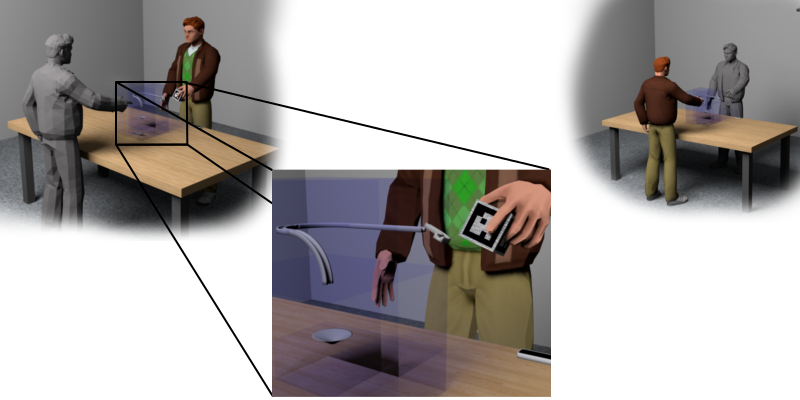
\includegraphics[width=1.00\textwidth]{figs/system_overview.png}
	\caption{Szenario der verteilten Kollaboration}
	\label{fig:system_overview2}
\end{figure}

